\documentclass{VUMIFPSkursinis}
\usepackage{algorithmicx}
\usepackage{algorithm}
\usepackage{algpseudocode}
\usepackage{amsfonts}
\usepackage{amsmath}
\usepackage{bm}
\usepackage{caption}
\usepackage{color}
\usepackage{float}
\usepackage{graphicx}
\usepackage{listings}
\usepackage{subfig}
\usepackage{wrapfig}
\usepackage{parcolumns}
\usepackage{enumitem}
\usepackage{array}
%PAKEISTA, tarpai tarp sąrašo elementų
\setitemize{noitemsep,topsep=0pt,parsep=0pt,partopsep=0pt}
\setenumerate{noitemsep,topsep=0pt,parsep=0pt,partopsep=0pt}
\renewcommand{\lstlistingname}{Kodo ištrauka}

% Titulinio aprašas
\university{Vilniaus universitetas}
\faculty{Matematikos ir informatikos fakultetas}
\department{Programų sistemų katedra}
\papertype{Kursinis darbas}
\title{WebAssembly panaudojamumo galimybių analizė kuriant internetines programas }
\titleineng{WebAssembly Usability Analysis in Web Development}
\status{3 kurso 5 grupės studentas}
\author{Kasparas Taminskas}
\supervisor{Lekt. Aurimas Šimkus}
\date{Vilnius – \the\year}

% Nustatymai
%\setmainfont{Palemonas}   % Pakeisti teksto šriftą į Palemonas (turi būti įdiegtas sistemoje)
\bibliography{bibliografija}

\begin{document}
\lstset{language=C}

% PAKEISTA	
\maketitle
\cleardoublepage\pagenumbering{arabic}
\setcounter{page}{2}

%TURINYS
\tableofcontents

\sectionnonum{Anotacija}
WebAssembly technologija — sėkmingai moderniose interneto naršyklėse realizuotas naujų, atvirų žiniatinklio standartų rinkinys, suteikiantis iki šiol neregėtus greitaveikos rodiklius ir naujas programavimo galimybes žiniatinklyje. Nepaisant to, technologija kol kas išlieka tik pradiniuose vystymo etapuose, plati žiniatinklio programuotojų bendruomenė tik pradeda susipažinti su jos galimybėmis. Dėl standarto naujovės dažnai pasigirsta tam tikrų mitų ar skambių pareiškimų, tokių kaip JavaScript kalbos gyvavimo pabaiga. Šiuo rašto darbu siekiama apžvelgti technologijos atsiradimo prielaidas, atskleisti jos paskirtį ir išanalizuoti pritaikymo galimybes tose situacijose, kuriose jos atrodo prasmingos. Įgyvendinus šiuos siekius, tikiu, pavyks sugriauti minėtas vyraujančias spekuliacijas apie šį naują standartą.

\sectionnonum{Įvadas}
Interneto naudojimo reikšmė per 30 paskutiniųjų metų nuo žiniatinklio atsiradimo išaugo 
eksponentiškai. Nors saityno potencialas buvo pastebimas nuo pat jo atsiradimo ir taikymo pradžios, tačiau vargu, ar 
kas nors XX a. IX dešimtmetyje galėjo pagalvoti, jog auganti interneto reikšmė pasieks tokį 
lygį, jog tradicinės programų sistemos, turinčios didžiulę kodo bazę, kuriamos skirtingoms 
fizinėms platformoms ir programinėms aplinkoms, reikalaujančios intensyvaus mašininių resursų 
panaudojimo, bus taip pat pasiekiamos tiesiog vienu pelės paspaudimu, nepriklausys nuo 
konkrečios mašininės architektūros, programinės aplinkos ir nereikalaus jokių specialių 
diegimo etapų.

Šiomis dienomis programinės įrangos kūrimo rinkoje internetinės technologijos ir 
platformos, debesų kompiuterija yra įmonių dėmesio centre, nes galimybė pasiūlyti programinį 
produktą internetu atveria didelį konkurencinį pranašumą – klientams nebereikia įsidiegti 
programinės įrangos į savo elektroninius įrenginius, užtenka vienos programos – interneto 
naršyklės – kuri atveria plačias galimybes naudotis skirtingų tipų programomis, pateikiamomis, 
kaip paslauga klientui (angl. — Software as a Service). Be to, patys programų sistemų kūrėjai 
patiria mažesnius kaštus kurdami ir palaikydami savo produktus, nes nebelieka poreikio turėti 
skirtingų kodo bazių specifinėms operacinėms aplinkoms ar įrenginiams.

Poreikis turėti kompleksiškas programų sistemas internetinėje erdvėje kelia didelius 
reikalavimus pagrindiniams saityno technologijų kūrėjams – didiesiems naršyklių gamintojams – 
kurių technologiniai sprendimai įgalina programuotojus įgyvendinti programinius sprendimus 
internete: šios naujos kartos programos internete turi užtikrinti tokius pačius kokybinius 
reikalavimus — greitaveiką, saugumą ir patikimumą — kaip senosios. Šioje vietoje susiduriama 
su dideliais technologiniais naršyklių variklių implementacijos ir pagrindinės internetinių 
technologijų programinės kalbos – JavaScript – ribojimais, neleidžiančiais įgyvendinti 
internetinių programų visiško supanašėjimo su tradicinėmis, veikiančiomis specifinėse 
platformose. 

WebAssembly standarto specfikacija ir jos formalus įgyvendinimas naršyklių 
smėliadėžės (angl. – sandbox) aplinkose siūlo sprendimą – binarinio formato kodo vykdymą 
greitaveikai imliose programų sistemų verslo logikos vietose papildant tradicinį JavaScript 
kodą. Ši technologinė naujovė, apibrėžta Pasaulinio žiniatinklio konsorciumo (W3C) ir palaikoma
visų modernių naršyklių kūrėjų, leidžia ženkliai sumažinti likusius techninius barjerus tarp 
naujos kartos internetinių programų sistemų ir tradicinių, nuo vykdymo aplinkos priklausomų 
sprendimų, todėl atveria saityne dar neišnaudotas rinkos perspektyvas, sėkmingai gyvuojančias
tradicinėse platformose. 

\sectionnonum{Tikslas ir uždaviniai}
Šio rašto darbo tikslas – pasiūlyti konkrečius praktinius variantus, kaip standartas 
gali būti integruotas į naujus ir jau egzistuojančius internetinius programinius sprendimus. 
Šie būdai leis programų sistemų kūrėjams išnaudoti stipriąsias technologijos puses ir taip 
įgauti didesnį konkurencinį pranašumą internetinėje programų sistemų rinkoje kuriant unikalias, nauju standartu paremtas programas ir tokiu būdu susikurti naują rinkos erdvę ar ją išplėsti. 

Pagrindiniai tarpiniai rašto darbo uždaviniai, padedantys atskleisti standarto esmę ir įgyvendinti užsibrėžtą tikslą:
\begin{itemize}
    \item Prielaidų, paskatinusių WebAssembly standartų rinkinį atsirasti, analizė
    \item WebAssembly standarto koncepcinės veikimo logikos suvokimas
    \item Skirtingų WebAssembly pritaikymo galimybių paieška
\end{itemize}

\section{Žiniatinklio ekosistemos technologinė raida}

Siekiant geriau suprasti dabartinę padėtį, kurioje buvo pristatytas WebAssembly standartas ir kokius poreikius jis patenkina, yra būtina apžvelgti viso žiniatinklio populiarumo augimą ir jo technologinę raidą.

\subsection{Interneto populiarumo augimas}

Interneto bendruomenę sudarančių Žemės gyventojų skaičius šiuo metu viršija pusę visos Žemės populiacijos. Šis augimas, prasidėjęs 1995 metais, kai Saitynas atsivėrė plačiai pasaulio bendruomenei, nesustoja ir toliau, tą galima pastebėti iš \ref{fig:internet_usage} paveikslėlyje matomos viešos metinės statistikos.

\begin{figure}[h!]
  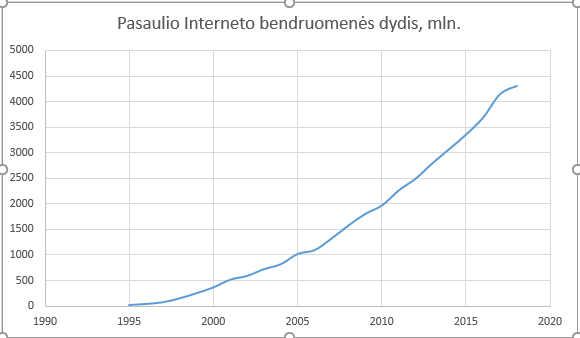
\includegraphics[scale=1]{interneto_naudojimo_statistika.png}
  \caption{Interneto bendruomenės narių skaičius 1995—2018 \cite{IWS19}}
  \label{fig:internet_usage}
\end{figure}

Ši statistika tik patvirtina plataus Interneto technologijų pritaikymo poreikio aktualumą ir didelę atsakomybę, tenkančią šių technologijų vedliams — interneto naršyklių kūrėjams. Žiniatinklis jau seniai nėra skirtas tik informacijos paieškai ir dalinimuisi, ką įgalino pradinės saityno technologijos — HTTP protokolas, HTML ir CSS žymėjimo kalbos. Šiuo metu vis didesnį pagreitį įgauna virtualios realybės, žaidimų industrijos, filmų ir muzikos sferų, neuroninių tinklų kūrimo ir analizės įrankiai. Deja, bet dažnai šių sprendimų pasiūlymas Internete būna ribotas dėl fundamentalių architektūrinių principų, kuriais paremtas programinio kodo vykdymas interneto naršyklėse.

\subsection{Programinio kodo vykdymas naršyklėse}
Interneto naršyklė architektūriniu požiūriu yra itin sudėtinga programa, nes procese nuo resurso parsiuntimo iš nutolusio serverio iki jo grafinio atvaizdavimo naršyklės lange dalyvauja daug sisteminių programos komponentų, nurodytų \ref{fig:browser_architecture} paveikslėlyje. 

\begin{figure}[h!]
  \begin{center}
  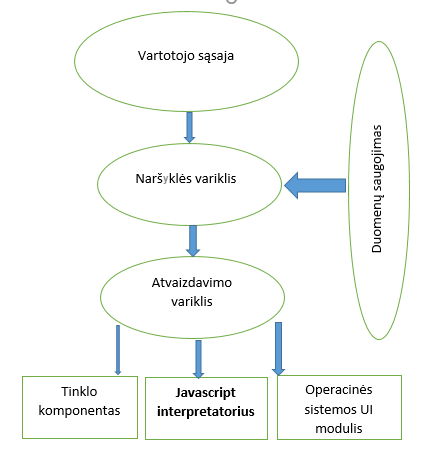
\includegraphics[scale=1]{naršyklės_architektūra.png}
  \end{center}
  \caption{Aukšto lygio interneto naršyklės veikimo principas \cite{MOR17}}
  \label{fig:browser_architecture}
\end{figure}

Vienas esminių šios schemos komponentų — JavaScript interpretatorius — žiniatinkliui suteikia dinamiškumą ir leidžia vykdyti skriptus, parašytus JavaScript programavimo kalba, tiesiog naršyklėje. Interpretatoriaus rezultatai siunčiami atvaizdavimo varikliui, kuris pasirūpina jų išdėstymu interneto programoje. \cite{MOR17} Norint geriau suprasti JavaScript vykdymo greitaveikos problemas, būtina suvokti interpretavimo trūkumus, todėl apžvelgsime du fundamentaliai skirtingus programinio kodo transliavimo į mašininį kodą principus.

\subsubsection{Transliavimo metodai}
Programinės kalbos dažniausiai skirstomos į statines ir dinamines, t.y. ar programiniai tipai egzistuoja kompiliavimo metu, ar yra nustatomi kodo vykdymo metu. Keletas šioms skirtingoms šeimoms priklausančių kalbų:
\begin{enumerate}
    \item Statinės: C, C++
    \item Dinaminės: Python, Rust, JavaScript
    \item Turinčios abejų šeimų požymių: Java, C\#
\end{enumerate} Pagal tai, kuriai šeimai kalba priklauso, skiriasi būdas, kuriuo išeities kodas yra verčiamas į mašinines tam tikros architektūros procesoriaus instrukcijas.

\subsubsubsection{Kompiliavimas ir interpretavimas}
\ref{tab:kompiliavimas_interpretavimas} lentelėje pateikti šių transliavimo metodų skirtumai ir ypatumai, atskleidžiantys konkretaus metodo privalumus ir trūkumus tam tikrose situacijose. Būtina pažymėti, kad universalaus sprendimo, kuris variantas geresnis, nėra, todėl programavimo pasaulyje derinami abu variantai.

\begin{table}[H]
  \centering
  \caption{kompiliavimo ir interpretavimo skirtumai \cite{PRO19}}
  {\begin{tabular}{|m{13em}|m{13em}|} \hline
     Kompiliavimo savybės & Interpretavimo savybės \\
    \hline
    Transliuojamas visas išeities kodas iš karto & Kodas transliuojamas dalimis 
 sakinys po sakinio \\
 \hline
 Pradinė kodo analizė 
     užima proporcingai didesnę laiko dalį, nei interpretavimo atveju, 
     tačiau vykdymas ženkliai greitesnis &
     Pradinis kodo analizės etapas daug greitesnis, 
     tačiau vykdymo greitaveika lėtesnė   \\
    \hline
     Generuojamas tarpinis objektinis kodas, kuris
 reikalauja surišimo žingsnio, papildomai naudojama atmintis & Nėra generuojama jokio tarpinio kodo \\
 \hline
 Klaidos pranešimas 
 generuojamas tik atlikus pilną kodo analizę, derinimo žingsnis daug sunkesnis &
 Programa transliuojama iki pirmos klaidos, kuomet 
 vykdymas stabdomas, todėl programos derinimas lengvas  \\
 \hline
  \end{tabular}}
  \label{tab:kompiliavimas_interpretavimas}
\end{table}

\subsubsection{JavaScript kalbos savybės}

Nuo pat žiniatinklio atsiradimo pradžios interneto technologijų branduolį sudaro JavaScript programavimo kalba, kurios prototipas per 10 dienų buvo sukurtas 1995 metais kompanijos Netscape Communications \cite{BAH15}. Ši programavimo kalba žiniatinklyje iki šiol užėmė visišką monopoliją, interneto aplikacijų klientinės dalies kūrimas be jos yra tiesiog sunkiai įsivaizduojamas atvejis. Kalbos populiarumą ir išplitimą patvirtina GitHub saugyklos repozitorijų statistiniai duomenys, pagal kuriuos kalba jau ilgą laiką pirmauja turėdama virš 320000 aktyvių repozitorijų. \cite{GIT19}

\subsubsubsection{Dinaminė prigimtis}

JavaScript programavimo kalba pasižymi dinaminiais tipais, t.y. kintamieji savo reikšmių tipus gali keisti skripto vykdymo metu. Žemiau pateikta kodo ištrauka yra visiškai validi ir leidžiama interpretatoriaus:

\begin{center}
\begin{small}
\begin{verbatim}
var x = 10;                   //console.log(x) => 10
x = "sveiki";                 //console.log(x) => sveiki
x = {                         //console.log(x) => [Object]
    a: "sveiki is objekto",
    b: 10,
    c: true
}
\end{verbatim}
\end{small}
\end{center}

Ši kalbos savybė programuotojams užtikrina lanksčias galimybes greitai ir ekspresyviai rašyti programinį kodą, kurio vykdymo pradžia yra itin greita, nes JavaScript yra interpretuojama kalba. Deja, bet ši kalbos dinamiškumo savybė itin trukdo vykdyti programinį kodą, kuris imlus operacijų kiekiui, reikalauja didelės greitaveikos, nes interpretatorius privalo kiekvieną kartą tikrinti, ar vykdomas kodas turi tuos pačius tipus, monitoringo procesas yra imlus greitaveikai. \cite{LCW17}

\subsubsection{Naršyklių gamintojų greitaveikos problemos sprendimas}

Didieji naršyklių gamintojai siekdami išnaudoti geriausias interpretatorių ir kompiliatorių savybes įdiegė naujus papildomus žingsnius JavaScript kodo vykdymo variklyje procese. Dauguma JavaScript variklių šiuo metu naudoja labai panašios architektūros kodo kompiliavimo procesus, todėl panagrinėsime vieno jų — Google kompanijos kuriamo ir palaikomo atviro kodo variklio — veikimo principus.

\subsubsubsection{V8 variklio JavasCript kodo vykdymo etapai}
Iki 2008 metų JavaScript kodo vykdymas naršyklėse buvo pastibimai lėtesnis, tačiau prasidėjus naršyklių gamintojų „greitaveikos karams" buvo įdiegti JIT (angl. — Just in Time) kompiliatoriai, kurie pastebimai padidino greitaveikos rodiklius. \cite{DAC17} Šių kompiliatorių vietą JavaScript kodo vykdymo grandinėje galima matyti \ref{fig:v8_pipeline} paveikslėlyje.

\begin{figure}[h!]
  \begin{center}
  \includegraphics[scale=0.8]{V8_kompiliavimo_grandinė.png}
  \end{center}
  \caption{Chrome naršyklėje naudojamo V8 JavaScript variklio kodo vykdymo grandinė \cite{HNO19}}
  \label{fig:v8_pipeline}
\end{figure}

JIT kompiliatoriai kodą optimizuoja pagal sukauptą informaciją iš monitoringo įrankio, kuris stebi kintamųjų tipus, jų kitimą, funkcijų kvietimo dažnius ir kt. Jeigu optmizuotas kodas tampa nevalidus (tarkime, jog atėjo nauji kintamųjų tipai), atliekamas deoptimizavimo žingsnis, JavaScript kodo vykdymas grąžinamas V8 interpretatoriui - Ignition. Šis procesas reikalauja laiko, todėl, žinoma, kenčia ir kodo vykdymo greitaveika, tačiau gana stabiliam kodui optimizavimo procesas labai naudingas.
\subsubsubsection{Ribojimai}
Nepaisant šių technologinių naujovių naršyklių varikliuose, optimizavimo procesas vykdant JavaScript kodą vis tiek dažnai neatitinka keliamų poreikių, reikalavimų. Tas puikiai matosi pritaikant vaizdo apdorojimo algoritmus, skirtus tam tikram efektui išgauti. Pavyzdžiui, kadrų skaičius per sekundę, JavaScript kalba realizavus Super Edge Inv vaizdo efekto algoritmą, yra pastebimai žemas ir juntamas aiškus uždelsimas. \cite{WVE17} Reikalinga naujovė, kuri leistų internete išgauti tokią pačią greitaveiką, kuri sėkmingai taikoma programuojant su tradicinėmis platformomis, pavydžiui, OpenGL grafine biblioteka ir statine kompiliuojama C++ kalba.

\section{WebAssembly standarto specifikacija}

WebAssembly yra standartų rinkinys, sukurtas ir palaikomas Pasaulio žiniatinklio konsorciumo (angl. — World Wide Web Consorcium), apibrėžiantis koncepcinį žemo lygio mašinio kodo formatą, į kurį gali būti verčiamos aukšto lygio programavimo kalbos. \cite{WAS17}

\subsection{Programavimo kalbos ypatybės}
WebAssembly yra žemo lygio, statinė programavimo kalba, turinti vos keletą kintamųjų tipų:

\begin{itemize}
    \item Sveikojo skaičiaus: i32, i64
    \item Slankaus kablelio: f32, f64
\end{itemize}
Lyginant šią kalbą su JavaScript, kuri yra dinaminė, aukšto lygio, galima pastebėti, jog nėra tokios įvairovės ir lankstumo — jokių eilučių tipų, masyvų, objektų. Funkcijų parametrų ir grįžimo reikšmės privalo būti griežtai deklaruotos ir apribrėžtos. Taip pat WebAssembly specifikacijoje apibrėžti statiniai užvardinti funkcijų importavimai ir eksportavimai.


\subsection{Koncepcinio mašininio kodo vykdymas}
WebAssembly mašininis kodas skirtas vykdyti steko pagrindu veikiančioms virtualioms mašinoms. Virtuali mašina yra aukšto lygio abstrakcijos sluoksnis, leidžiantis programinį kodą vykdyti skirtingose operacinėse sistemose ir fizinėse architektūrose, todėl WebAssembly mašininį kodą lyginti su tradiciniu konkrečios fizinės architektūros mašininiu kodu būtų neteisinga. \cite{DAC17} Supaprastinta WebAssembly programinio kodo vertimo į konkrečią fizinę architekūrą schema pateikta \ref{fig:wasm_compilation} paveikslėlyje. Programinės kalbos dažnai turi tarpines kodo išraiškas (angl. — Intermediate Representation), skirtas programinį kodą versti į konkrečios fizinės architektūros mašinininį kodą. WebAssembly mašininis kodas sugeba priimti šį tarpinį formatą, naršyklių implementacijos sugeba atlikti WebAssemly kodo transliavimą į konkrečią fizinę architektūrą be sudėtingų ir laikui imlių žingsnių. 

\begin{figure}[h!]
  \begin{center}
  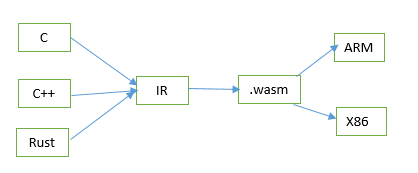
\includegraphics[scale=1]{webassembly_kompiliavimas.png}
  \end{center}
  \caption{WebAssembly kodo kompiliavimas \cite{LCW17}}
  \label{fig:wasm_compilation}
\end{figure}

\subsection{Virtualios mašinos realizacija}

WebAssembly formatas sukurtas steko pagrindu veikiančiai mašinai — tai specialus virtualios mašinos implementacijos atvejis, kai aritmetiniai ir loginiai operandai ir operacijų rezultatai saugomi steko pagrindo duomenų struktūroje, o išėmimo ir įdėjimo tvarka grįsta LIFO (angl. — last-in-first-out) principu. 

\begin{figure}[h!]
  \begin{center}
  \includegraphics[scale=1]{sudėtis_steke.png}
  \end{center}
  \caption{Sudėtis steke}
  \label{fig:stack_addition}
\end{figure}

Šis virtualios mašinos implementacijos būdas užtikrina efektyvią greitaveiką, nes nereikia išreikštinai žinoti operandų atminties adresų — naudojama steko viršūnės rodyklė (angl. — Stack Pointer), o kiekiena įdėjimo/išėjimo operacija pakeičia šios rodyklės reikšmę vienetu.
Kaip matome \ref{fig:stack_addition} paveikslėlyje, paprastai sudėties operacijai steko implementacijos atveju reikia keturių komandų. Egzistuoja registrais grįsta virtualios mašinos realizacija, kurioje sudėtis gali būti išreiškiama viena operacija, tačiau tokiu atveju reikia nurodyti ir žinoti registrų adresus. \cite{MSS12} Neteisinga teigti, jog viena implementacija universaliu atveju geresnė už kitą, efektyvumą lemia naudojimo kontekstas.

\subsection{Atviras standartų rinkinys}
WebAssembly technologija yra standartizuota, todėl nereikalauja papildomų įskiepių ar kitų programinių papildinių. Visos modernios naršyklės - Chrome, Safari, Edge, Firefox - realizavusios WebAssembly vykdymo variklius, todėl programuotojams nebereikia spręsti skirtingų naršyklių suderinamumo problemos, kuri dažnai itin išaugina programavimo laiko ir kainos kaštus. Tiesa, reikia paminėti, jog šis standartas nepalaikomas Internet Explorer naršyklėse. 
\section{WebAssembly panaudojamumo būdai}
Standarto panaudojimo galimybes kuriant interneto programas galima skirstyti pagal pritaikymo skalę — kokį proporcinį visos programos kiekio dalį užima WebAssembly kodo bazė.

\subsection{Modulio integracija į egzistuojantį JavaScript projektą}
Dar iki WebAssembly standarto atsiradimo, nuo ECMAScript2015 standarto specifikacijos išleidimo, JavaScript ekosistema tapo daug moduliaresnė, nei buvo prieš tai. Ši technologinė savybė leidžia enkapsuliuoti realizacijos logiką, o klientui pateikti tik ribotą programinę sąsają (angl. — Application Programming Interface), skirtą naudotis paketu ar moduliu. WebAssembly standartas kuriamas atsižvelgiant į modulių naudą ir poreikį.

\subsubsection{Problemos apibrėžimas}
Sakykime, jog turime realizavę internetinę programą, kurios esminė verslo logikos dalis atlieka procesoriaus ar vaizdo plokštės darbo laikui imlias operacijas. Mūsų klientai džiaugiasi, jog esame pirmieji realizavę tokio tipo sistemą internete, tačiau skundžiasi, jog darbas su sistema nėra sklandus, juntamas dažnas uždelsimas. Tokių sistemų pavyzdžiai galėtų būti vaizdo, garso kodavimo ir apdorojimo programos, papildytos realybės (angl. — Augmented Reality) sprendimai, dirbtinio intelekto sistemos. 
\subsubsection{Sprendimas}
Galima bandyti susidariusią problemą spręsti pertvarkant egzistuojantį centrinį verslo logikos algoritmą, parašytą JavaScript programavimo kalba ir stebint greitaveikos rodiklius, tačiau anksčiau ar vėliau neabejotinai bus pasiekta riba, kurios peržengti su esama technologija nebus įmanoma, nes pati kalba nesuteikia prieigos prie žemų programinių konstruktų, tokių kaip savarankiškas ir efektyvus atminties išskyrimas ir valdymas. 
\subsubsubsection{WebAssembly integracija}
Šioje vietoje atsiranda galimybė panaudoti enkapsuliuotą WebAssembly modulį, kuris savyje turėtų realizuotą centrinį skaičiavimų logikos algoritmą. Jeigu mūsų internetinės programų sistemos sprendimas kilo iš jau anksčiau egzistavusios darbalaukinės programos, didelė galimybė, jog mums net nereikės perrašinėti jokios verslo logikos kita kalba, galėsime sukompiliuoti seną kodo bazę į \verb|.wasm| mašininio kodo formatą ir iškviesti programinį modulį tiesiai iš interneto naršyklės. Šis seno kodo perpanaudojimo principas suteikia galimybę išnaudoti WebAssembly technologinės naujovės teikiamą naudą net nemokant programuoti tomis kalbomis, kurių bibliotekas ar modulius norime panaudoti. Sakykime, jog savo algoritmą turime įgyvendinę C programavimo kalba, imituokime mūsų verslo logikos funkcionalumą realizuodami paprastą Burbulo metodo (angl. — Bubble Sort) rikiavimo funkciją:

\begin{center}
\begin{small}
\begin{verbatim}
int8_t* EMSCRIPTEN_KEEPALIVE bubbleSort(int8_t *buf, int n) {
    for (int i=0; i<n—1;i++) {
        for (int j=0;j<n—i—1;j++) {
            if (buf[j]>buf[j+1]) {
                swap(&buf[j], &buf[j+1]);
            }
        }
    }
    return buf;
}
\end{verbatim}
\end{small}
\end{center}

Verta paminėti, jog \verb|EMSCRIPTEN_KEEPALIVE| direktyva nurodo, jog šią funkciją reikia įtraukti į WebAssembly eksportuojamų funkcijų sąrašą, tuomet ją bus galima kviesti tiesiai iš JavaScript programinio kodo. \cite{EMD17}

Kai jau turime parašę savo centrinį verslo logikos algoritmą, esminis žingsnis — šį išeities kodą paversti binariniu \verb|.wasm| formato moduliu, kurį galėtume importuoti naršyklėse. Patogiausias ir plačiausiai taikomas rinkoje įrankis — Emscripten atviro kodo kompiliatorius. Savo darbalaukinėje sistemoje sudiegę šį įrankį, komandinėje eilutėje galime iškviesti kompiliavimo komandą:

\begin{center}
\begin{small}
\begin{verbatim}
emcc bubble_sort.c —s WASM=1 —s EXPORTED_FUNCTIONS="['_bubbleSort']" 
—s "EXTRA_EXPORTED_RUNTIME_METHODS=['ccall','cwrap']"
\end{verbatim}
\end{small}
\end{center}

Kompiliavimo komandos sintaksė skiriasi priklausomai nuo naudojamos operacinės sistemos, šiuo atveju buvo naudojama Windows 10 operacinė sistema ir jos komandinė eilutė.

Įvykdžius terminalo lango komandą įrankis sugeneruoja \verb|.wasm| modulį ir \verb|.js| failą, kuris skirtas inicijuoti WebAssembly modulio vykdymą naršyklėje. Naršyklių gamintojai teigia, jog planuose yra patogesnis \verb|.wasm| modulio integravimas taikant tradicinį modulių importavimo požiūrį: \verb|<script type="module"></script>|. Deja, tačiau rašymo metu ši galimybė dar neegzistuoja, todėl modulio užkrovimas naršyklėje reikalauja gana didelio kiekio surišančiojo JavaScript kodo, kurį sugeneruoja minėtasis Emscripten įrankis.

Šiame pavyzdyje C funkcijai iš JavaScript kodo turime perduoti masyvą ir jo elementų ilgį, kad galėtume per jį iteruoti. Kol kas tiesioginis parametrų perdavimas galimas tik su primityviaisiais skaitiniais tipais, jeigu norime perduoti masyvą, turime pasitelkti piramidės struktūrą (angl. — Heap Data Strcuture). 
\begin{figure}[h!]
  \begin{center}
  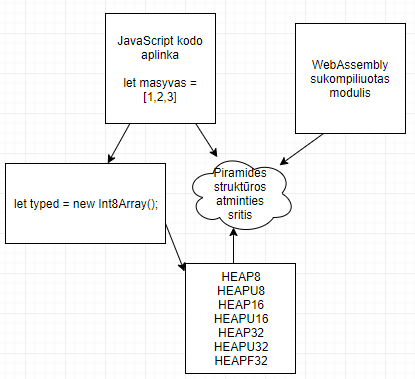
\includegraphics[scale=1]{wasm_heap.png}
  \end{center}
  \caption{WebAssembly ir JavaScript komunikacija naudojant piramidės atmintį}
  \label{fig:wasm_stack}
\end{figure}
Ši atminties sritis WebAssembly standarte yra tiesiog paprastas JavaScript objektas, kuris imituoja tradicinę C/C++ kalbų piramidės duomenų struktūrą, nes pastarosios pasiekti dėl saugumo priežasčių programuotojai galimybės neturi. 
Sudėtingų tipų perdavimą tarp JavaScript kodo ir WebAssembly modulio galima pavaizduoti \ref{fig:wasm_stack} paveikslėlyje nurodyta schema, kurioje matosi, jog komunikacija tarp aplinkų vyksta netiesiogiai, žiūrint į bendrą atminties sritį.

Svarbu paminėti, jog negalime į piramidę tiesiogiai patalpinti apibrėžto JavaScript masyvo, turime jį paversti į tipizuotą masyvo tipą, atitinkantį konkretaus tipo piramidę, nes vieno tipo piramidėje negalima laikyti skirtingo tipo duomenų — kitu atveju bus gaunami netikėti ir nesąmoningi rezultatai. 

Taigi, turėdami sukompiliuotą modulį ir jį iškviečiantį sugeneruotą surišantįjį JavaScript kodą, galime bandyti iškviesti aprašytą C rikiavimo funkciją iš naršyklės. Šiam tikslui naudojame integruotas WebAssembly standarto realizacijos \verb|Module.ccall()| ir \verb|Module.cwrap()| funkcijas, leidžiančias perduoti parametrus į WebAssembly modulį ir grąžinti rezultatą į JavaScript aplinką atgal. Šiame pavyzdyje naudojame \verb|wasm—arrays.js| atviro kodo biblioteką, patalpintą GitHub saugykloje, kuri suteikia papildomą \verb|ccall| ir \verb|cwrap| funkcijų abstrakcijos lygmenį, skirtą patogesniam naudojimui. \cite{WAA19} Taigi, naršyklės kode galime iškviesti mūsų rikiavimo funkciją perduodami skaičių masyvą:

\begin{center}
\begin{small}
\begin{verbatim}
        const res = ccallArrays(
          "bubbleSort",
          "array",
          ["array"],
          [[2, 1, 13, 4, 50]],
          { heapIn: "HEAP8", heapOut: "HEAP8", returnArraySize: 5 }
        );
        console.log(res);
\end{verbatim}
\end{small}
\end{center}

Pirmuoju parametru nurodome kviečiamą funkciją, antrasis parametras apibrėžia iš kviečiamos funkcijos grįžtantijį tipą, trečias ir ketvirtas — perduodamų parametrų tipus ir reikšmes, penktasis parametras — perduodamas objektas — apibrėžia jog naudosime WebAssembly \verb|HEAP8| (baito dydžio) sveikųjų skaičių piramidės atminties sritį. Įvykdžius \verb|ccallArrays| funkciją rezultato kintamasis \verb|res| gauna \verb|int8_t| tipo rodyklę, būtent tokio tipo, kokį apibrėžėme C funkcijoje. Ši rodyklė rodo į surikiuoto masyvo pradžios atminties sritį, todėl JavaScript kode galime pasiekti pakeistąjį masyvą. Našyklės konsolėje stebimas paveikslėjyje matomas kvietimo rezultatas.

\begin{figure}[h!]
  \begin{center}
  
\includegraphics[scale=1]{sorted_array.png}
  \end{center}
  \caption{Rezultatas naršyklės konsolės lange}
  \label{fig:sorted_array}
\end{figure}

Tagi, šiame pavyzdyje sugebėjome realizuoti logikos algoritmą C programavimo kalba, jį sukompiliuoti į WebAssembly modulį ir iškviesti JavaScript kode. Ši situacija parodo, jog WebAssembly standarto moduliarumo savybė leidžia skaičiavimams jautrias logikos sritis perkelti iš JavaScript kodo į WebAssembly modulius. Būtent todėl WebAssembly standartas ne pakeičia, o papildo JavaScript veikimą ten, kur pokytis atrodo racionalus ir reikalingas.

\subsubsection{Realaus pasaulio scenarijai}

Aprašytasis pavyzdys tik vaizdžiai parodo, kaip galima WebAssembly integruoti į egzistuojančią interneto sistemą pagerinant greitaveikos rodiklius. Taikant šį principą rinkoje galima paspartinti jau egzistuojančius sprendimus.

Vienas tokių atvejų galėtų būti ReactJS biblioteka, skirta kurti klientiniam interneto kodui. Esminis šios bibliotekos suderinimo (angl. — Reconciliation) algoritmas, skirtas efektyviai perpiešti DOM medį ir pastebėti, kurie šio medžio lapai pakeitė būseną, galėtų būti pakeistas WebAssembly realizacijos kodu išlaikant tokį patį programinį kontraktą React bibliotekos naudojams (angl. — API). Tokiu atveju vienintelis pokytis, kurį pajustų naudotojai — išaugusi bibliotekos veikimo sparta .

Kitas pavyzdys, kuris rinkoje jau implementuotas — kompanijos eBay programuotojų komandos sukurta internetinė brūkšninio kodo nuskaitymo programa, skirta eBay aukciono pardavėjams įkelti savo parduodamas prekes. Šis įrankis eBay programuotojų buvo sukurtas C++ kalba ir sėkmingai veikė iOS ir Android mobiliose aplinkose. Atsiradus WebAssembly technologijos realizacijai interneto naršyklėse, eBay programuotojai egzistuojančią kodo bazę sukompiliavo į \verb|.wasm| modulį, rezultatas buvo stebinantis — lyginant su anksčiau veikusiu JavaScript brūkšninio kodo nuskaitymo įrankiu, kuris veikdavo vieno kadro per sekundę režimu, WebAssembly realizacija leido pasiekti 50 kartų didesnę greitaveiką. \cite{NHT19}

\subsection{Naujo karkaso kūrimas WebAssembly pagrindu}
Vienas didžiausių standarto privalumų, kuro įtaką žiniatinkliui galima laikyti revoliucine, yra tai, jog WebAssembly mašininio kodo formatas skirtas būti kompiliuojamu iš skirtingų programavimo kalbų. Tai reiškia, jog JavaScript kalbos monopolis kuriant klientines interneto programas baigėsi. Anksčiau kuriant klientinę žiniatinklio sistemos dalį buvo būtina turėti plačias JavaScript kalbos ir ja parašytų karkasų ir bibliotekų, tokių kaip React, Angular, Vue žinias. Neteisinga teigti, jog JavaScript žinių nuo šiol nebereiks, tačiau žiniatinklyje vis daugiau vietos atsiras ir kitoms programavimo kalboms, kurias buvo įprasta matyti programuojant serverinę sistemos dalį.

Šis WebAssembly pritaikymo pavyzdys yra daug platesnis nei anksčiau aprašytasis centrinės logikos realizacijos pakeitimo, nes apima visą klientinės programos logikos perkėlimą į WebAssembly mašininį kodą.

Naujo karkaso kūrimo galimybes ir iššūkius naudojant WebAssembly kodą galima suprasti įsigilinus į jau realizuotus pavyzdžius, kurie, nors vis dar ankstyvose stadijose, tačiau jau nusako kryptį, kurios bus laikomasi.

\subsubsection{Microsoft .NET Blazor karkasas}
Microsoft kompanijos kuriamas .NET Blazor produktas — vartotojo sąsajos kūrimo C \# programavimo kalba karkasas, leidžiantis .NET programos kodui būti vykdomam tiesiogiai naršyklėje. \cite{BLZ19} Ši savybė leidžia programuotojams pernaudoti serverio dalyje esantį .NET kodą kuriant klientines programas.
\subsubsubsection{Platformos koncepcinė architektūra}
C \# kalbos kodo vykdymui reikalinga .NET vykdomoji aplinka, todėl esminis Blazor karkaso funkcinis vienetas yra Microsoft Xamarin komandos kuriama ir palaikoma Mono .NET vykdomoji aplinka, skirta mobiliųjų programėlių ir žaidimų konsolinėms platformoms kūrimui naudojant .NET technologijas. Nuo šiol ši vykdomoji aplinka veikia ir interneto naršyklėse — pastaroji buvo sukompiliuota į WebAssembly modulį. Šis modulis su savimi turi ir nebenaudojamų resursų surinkimo konstruktą (angl. — Garbage Collection), leidžiantį programuotojui nesirūpinti rankiniu atminties valdymu programuojant. Aukšto lygio Blazor veikimo principas nurodytas \ref{fig:blazor_architecture} schemoje, kur matome, jog mono.wasm — tai į WebAssembly mašininio kodo formatą sukompiliuota .NET Mono vykdomoji aplinka.

\begin{figure}[h!]
  \begin{center}
  \includegraphics[scale=0.9]{blazor_veikimo_architektūra.png}
  \end{center}
  \caption{Blazor karkaso veikimas naršyklėje \cite{BLZ19}}
  \label{fig:blazor_architecture}
\end{figure}

Verta paminėti, jog, kaip ir praeitame skyriuje demonstruotame pavyzdyje, kur buvo naudojamas Emscripten pagalba sugeneruotas JavaScript kodas, reikalingas užkrauti WebAssembly moduliui, turime \verb|mono.js| ir \verb|blazor.js| skriptus, reikalingus vykdomosios \verb|mono.wasm| aplinkos užkrovimui. Šis .NET vykdomomios Mono aplinkos režimas yra interpretuojamasis, nes mūsų kurta programa \verb|Programa.dll| nėra sukompiliuota į WebAssembly mašininį formatą, o interpretuojama pačioje kliento naršyklėje \verb|mono.wasm| modulio. Mono aplinka palaiko ir išankstinį (angl. — Ahead of Time) programos vykdymo būdą, kai mūsų kurta programa sukompiliuoajama į WebAssembly modulį iš anksto. Kaip pirmame skyriuje minėta, nėra fundamentaliai aišku, kuris modelis geresnis, tačiau interpretuojamas modelis daug artimesnis programavimui internete, nes kodo pokyčiai atsispindi naršyklės lange beveik iš karto — sukompiliavus pakeistą programos vietą, o taikant išankstinį modelį kompiliavimo žingsnis užtrunka pastebimai ilgiau, tačiau pats veikimo greitis greitaveikai jautriose vietose būna didesnis.

\subsubsubsection{Razor sintaksė Blazor klientinių žiniatinklio programų kūrime}
Faktas, jog visa klientinė programos logika perkeliama vykdyti į WebAssembly modulius leidžia beveik išsisukti be JavaScript kodo rašymo jį pakeičiant .NET pasaulyje gerai žinomai Razor sintaksei, kuri sujungia HTML, CSS žymėjimo kalbas ir C \# sintaksę viename išeities kodo dokumente:

\begin{center}
\begin{small}
\begin{verbatim}
@page "/skaitliukas"
<p>Dabartinis skaicius: @currentCount</p>
<button onclick="@IncrementCount">Padidinti</button>
@functions {
    int currentCount = 0;
    void IncrementCount()
    {
        currentCount++;
    }
}
\end{verbatim}
\end{small}
\end{center}

Pateiktame pavyzdyje parodyta \verb|<Counter>| vartotojo sąsajos komponento logika, kurioje paspaudus mygtuką skaitliukas padidinamas vientu. Dažniausiai tokį kodą dinamiškai vykdo JavaScript variklis, tačiau, kaip matome iš pavyzdžio, viskas rašoma naudojant tik HTML ir C \#, šiame pavyzdyje nedaroma jokių HTTP užklausų į nutolusį serverį. Direktyva \verb|@page| nurodo maršrutą, kuriuo bus pasiekamas komponentas.

\subsubsubsection{Blazor karkaso iššūkiai}
Kuriant serverio pusės logiką ASP.NET technologine platforma nebuvo itin aktuali surinkimo tekstų (angl. — .NET assemblies) užimama disko vieta serveryje — 2 MB ar 50 MB disko vietos užimantis kodas didelio skirtumo nedarydavo, tačiau naršyklės vykdyme šis aspektas yra kritinis, todėl net pritaikius Mono vykdomosios aplinkos ir programos kešavimo mechanizmą, yra itin svarbu, jog pirmasis puslapio užkrovimas, kurio metu parsiunčiama vykdomoji aplinka ir programinis kodas, būtų greitas. Technologijos kūrėjai pripažįsta, kad Blazor programa nesugebės pasiekti tokio suspaudimo lygio, kokį sugeba išgauti ReactJS biblioteka, tačiau pritaikius kelis optimizavimo metodus pasiekiamas rezultatas, leidžiantis galutiniam vartotojui sklandžiai naudotis klientine programa. Keli iš tų metodų yra:
\begin{itemize}
    \item HTPP užklausų atsakymų suspaudimas
    \item Kompiliavimo metu .NET IL surišiklis (angl. — Intermediate Language linker) statiškai skenuoja visą kodą ir pašalina tas dalis, kurios bus nenaudojamos kodo vykdymo metu
    \item .NET vykdomoji aplinka ir programos surinkimo failai kešuojami naršyklėje, kad nereiktų daryti nereikalingų užklausų į nutolusį serverį
\end{itemize}

\sectionnonum{Rezultatai ir išvados}
Rašto darbe pristatyta žiniatinklio naudojimo augimo tendencija, atskleistos JavaScript kalbos ir naršyklių variklių kodo vykdymo architektūrinės greitaveikos problemos, lėmusios WebAssembly standarto sukūrimą. Taip pat darbe suformuluotas standarto apibrėžimas ir pristatyta jo veikimo logika, nurodyta koncepcinė WebAssembly veikimo naršyklėse architektūra. Šiame darbe pristatyti du pagrindiniai WebAssembly panaudojimo scenarijai: centrinio greitaveikai imlios verslo logikos modulio pakeitimas WebAssembly modulio realizacija ir kitas - naujos klientinės programos kūrimas nuo pradžių pasitelkiant karkasus, sukurtus WebAssembly technologijos pagrindu ir leidžiančius interneto platformoje programuoti kitomis programavimo kalbomis, nei JavaScript. Rašant šį rašto darbą teko išbandyti C kalba parašytos burbulo metodo rikiavimo funckijos kompiliavimo į WebAssembly modulį procesą ir iškviesti sukompiliuotą kodą iš naršyklės perduodant parametrus iš JavaScript aplinkos  į WebAssembly kodą, todėl praktiškai buvo įsitikinta panaudojimo galimybėmis jau šiomis dienomis, su egzistuojančiomis technologijomis

WebAssembly standarto atsiradimas ir pritaikymas neabejotinai turi savo panaudojimo galimybes ir vietas, kurios leidžia įmonėms patobulinti savo turimus programų sistemų produktus greitaveikos atžvilgiu ir taip įgauti dar didesnį klientų pasitikėjimą ir palankumą internete arba užimti naujas, dar nerealizuotas rinkos galimybes. Daugelis apie šį standartų rinkinį kalbančių žmonių net neabejoja, jog WebAssembly per pastaruosius kelis metus visiškai pakeis požiūrį, kaip kursime klientines žiniatinklio programas ir aš, susipažinęs su pristatyta technologija, negaliu su jais nesutikti, tačiau tikiuosi, jog šiuo rašto darbu taip pat pavyko skaitytojus įtikinti, jog WebAssembly technologija, kaip vaizduoja jos logotipas, tėra viena dėlionės dalis, papildanti - ne pakeičianti - kitą, tradicinę - JavaScript interneto pusę - tose vietose, kuriose pastaroji buvo ilgą laiką labai ribota.
%% PAKEISTAS PAVADINIMAS Į 'Šaltiniai'
\addcontentsline{toc}{section}{Šaltiniai} 
\printbibliography[heading=bibintoc, title=Šaltiniai]  % Šaltinių sąraše nurodoma panaudota
\begin{thebibliography}{99}

\bibitem[IWS19]{IWS19} 
Internet Growth Statistics, Žiūrėta[2019—06—07].  Prieiga internetu: \url{https://www.internetworldstats.com/emarketing.htm/}

\bibitem[LCW17]{LCW17} 
Lin Clark. A cartoon intro to WebAssembly, 2017. Žiūrėta [2019—06—07].  Prieiga internetu: \url{https://hacks.mozilla.org/2017/02/a—cartoon—intro—to—webassembly/}

\bibitem[MOR17]{MOR17} 
Monica Raghuwanshi. How does web browsers work?, 2017. Žiūrėta [2019—06—07].  Prieiga internetu: \url{https://medium.com/@monica1109/how-does-web-browsers-work-c95ad628a509}

\bibitem[PRO19]{PRO19} 
Interpreter Vs Compiler : Difference Between Interpreter and Compiler. Žiūrėta [2019—06—07].  Prieiga internetu: \url{https://www.programiz.com/article/difference-compiler-interpreter}

\bibitem[GIT19]{GIT19} 
A Small Place to Discover Languages In GitHHub. Žiūrėta [2019—06—07].  Prieiga internetu: \url{https://githut.info/}

\bibitem[DAC17]{DAC17} 
Dan Callahan: Practical WebAssembly, 2017. Žiūrėta [2019—06—07].  Prieiga internetu: \url{http://2017.jsconfbp.com/speakers/dan-callahan/}

\bibitem[HNO19]{HNO19} 
Yotam Kadishay. JavaScript V8 Engine Explained, 2019. Žiūrėta [2019—06—07].  Prieiga internetu: \url{https://hackernoon.com/javascript-v8-engine-explained-3f940148d4ef/}

\bibitem[WVE17]{WVE17} 
WebAssembly Video Editor, 2017. Žiūrėta [2019—06—07].  Prieiga internetu: \url{https://d2jta7o2zej4pf.cloudfront.net/}

\bibitem[WAS17]{WAS17} 
WebAssembly Documentation, High Level Goals 2017. Žiūrėta [2019—06—07].  Prieiga internetu: \url{https://webassembly.org/docs/high-level-goals/}

\bibitem[MSS12]{MSS12} 
Mark Sinnathamby. Stack based vs Register based Virtual Machine Architecture, and the Dalvik VM, 2012. Žiūrėta [2019—06—07].  Prieiga internetu: \url{https://markfaction.wordpress.com/2012/07/15/stack-based-vs-register-based-virtual-machine-architecture-and-the-dalvik-vm/}

\bibitem[EMD17]{EMD17} 
Emscripten Documentation. Building to WebAssembly. Žiūrėta [2019—06—07].  Prieiga internetu: \url{https://emscripten.org/docs/compiling/WebAssembly.html}

\bibitem[WAA19]{WAA19} 
DanRuta. wasm-arrays. Žiūrėta [2019—06—07].  Prieiga internetu: \url{https://github.com/DanRuta/wasm-arrays}

\bibitem[NHT19]{NHT19} 
Nick Heath, TechRepublic. Replacing JavaScript: How eBay made a web app 50x faster by switching programming languages. Žiūrėta [2019—06—07].  Prieiga internetu: \url{https://www.techrepublic.com/google-amp/article/replacing-javascript-with-webassembly-how-ebay-made-a-web-app-50x-faster-by-switching-programming-languages/?fbclid=IwAR0u8eTYgjIEVUxt6wA0Cu9PIo7kjcBUhxtYi849vNTk4TOB-L3m7tOGrho}

\bibitem[BLZ19]{BLZ19} 
Blazor Documentation. Žiūrėta [2019—06—07].  Prieiga internetu: \url{https://docs.microsoft.com/lt-lt/aspnet/core/blazor/?view=aspnetcore-3.0}

\bibitem[W3C19]{W3C19} 
Pasaulinio žiniatinklio konsorciumo svetainė Žiūrėta [2019—06—07].  Prieiga internetu: \url{https://www.w3.org/wiki/Main_Page}

\bibitem[BAH15]{BAH15} 
Ben Aston. A brief history of JavaScript. Žiūrėta [2019—06—07].  Prieiga internetu: \url{https://medium.com/@benastontweet/lesson-1a-the-history-of-javascript-8c1ce3bffb1}
\end{thebibliography}
% literatūra, kitokie šaltiniai. Abėcėlės tvarka išdėstomi darbe panaudotų
% (cituotų, perfrazuotų ar bent paminėtų) mokslo leidinių, kitokių publikacijų
% bibliografiniai aprašai.  Šaltinių sąrašas spausdinamas iš naujo puslapio.
% Aprašai pateikiami netransliteruoti. Šaltinių sąraše negali būti tokių
% šaltinių, kurie nebuvo paminėti tekste.

\sectionnonum{Sąvokų apibrėžimai}

\textbf{Programa kaip paslauga (angl. Software as a Service)} - programinis produktas, nereikalaujantis, jog vartotojas jį įdiegtų į savo elektroninį įrenginį, dažniausiai veikiantis paskirstytuose dalykiniuose serveriuose, duomenų centruose, galintis vienu metu aptarnauti daug vartotojų.

\textbf{Naršyklės smėliadėžės aplinka (angl. browser sandbox environment)} - naršyklėse įdiegta, izoliuota JavaScript ir WebAssembly kodo vykdymo erdvė, ribojanti prieigą prie sisteminių resursų siekiant apsaugoti galutinį interneto naršyklės naudotoją.

\textbf{Pasaulinio žiniatinklio konsorciumas (W3C)} - tarptautinis programinės įrangos kūrimo bendruomenės susivienijimas, kuriantis ir teikiantis standartus ir rekomendacijas žiniatinkliui. \cite{W3C19}

\textbf{HTTP protokolas (angl. Hyper Text Transfer Protocol)}

\textbf{HTML kalba (angl. Hyper Text Markup Language)}

\textbf{CSS kalba (angl. Cascading Style Sheets)}
TODO


\end{document}
